\section{Goals} \label{design-goals}

The goal here is to provide a zero-copy, in-memory, eventually
consistent key-value store using kernel bypassing to support high
throughput as well as low latency. The zero-copy property will allow
our latency to remain the same regardless of the sizes of keys and
values, though we can't say the same for the throughput since we will
be limited by the capacity of the NIC in term of raw bandwidth.

Providing low latency and high throughput requires every component of
the system to be fast and zero-copy. We therefore need a fast
networking stack and obviously a high-performance and concurrent
hashmap to store key-value entries as well as an efficient way to
interface with the network interface controller that will send our
packets on the wire. The choice of the networking protocol to transmit
requests and responses is also quite important since it will be the
central part of the system and will determine how much processing is
necessary to receive and send packets.

But creating a fast system is only part of the goal here. The
networking code should be re-usable in order to facilitate further
development of safe high-performance networking
applications in Rust. Providing a convenient and clear API to the
networking stack is therefore also a design goal. That means the API
should follow idiomatic Rust interface design principles and leverage
all the language features necessary to make it re-usable and generic.

The design of the system as a whole, as well as how each component
interface with the others is shown in
figure~\ref{fig:design-overview}.

\begin{figure}[htb!]
  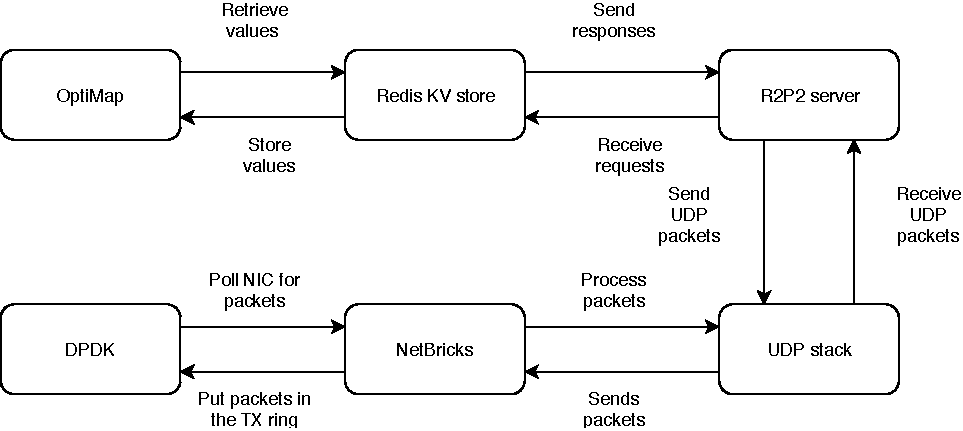
\includegraphics{../diagram/overview.pdf}
  \caption{System design overview}
  \label{fig:design-overview}
\end{figure}

\section{Local store} \label{sec:local-store-design}

The central component of any key-value store is an efficient
datastructure to store and retrieve values by their keys. Since we
also aim to provide true zero-copy semantics, this datastructure
should also avoid copying data around. Moreover, it should allow
values to be retrieved and used concurrently with minimum overhead.
A way to make values live outside of the store should also be provided
in order to permit said values to be held in the networking stack
after having been removed from the store.

With all these constraints in mind, we go with the design shown
in~\hyperref[fig:hashmap]{figure~\ref{fig:hashmap}}. The top level
table is a contiguous array of atomic pointers to overflow
buckets. And in turn each overflow bucket entry? is a pointer to a
key-value pair structure allowing fast, easy and zero-copy retrieval
of values.

\begin{figure}[htb!]
  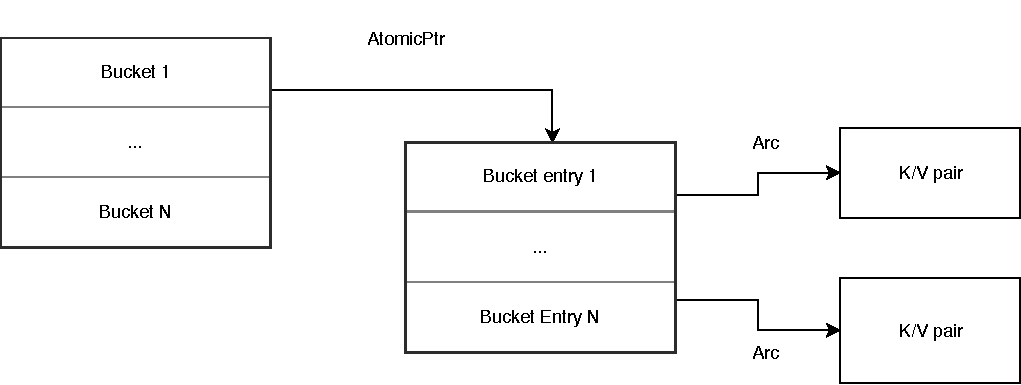
\includegraphics[width=\textwidth]{../diagram/amap1.pdf}
  \caption{Hashmap overview}
  \label{fig:hashmap}
\end{figure}

To satisfy the constraints, each pointer inside each overflow bucket,
as well as the pointers to the overflow buckets themselves are
atomically reference counted. Since our key-value store will use many
threads working concurrently to satisfy requests an atomic reference
count is necessary to avoid race conditions when updating the
reference count. But more importantly an atomic reference count allows
values to be removed from the store while still being used elsewhere,
as shown
in~\hyperref[fig:value-sharing]{figure~\ref{fig:value-sharing}}.

\begin{figure}[htb!]
  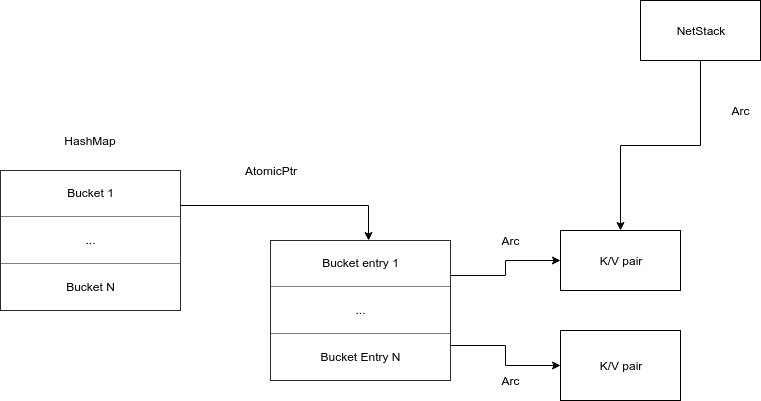
\includegraphics[width=\textwidth]{../diagram/cc1}
  \caption{Value sharing}
  \label{fig:value-sharing}
\end{figure}

% \marios{Pick 1,2 cases such as an update and a delete and walk the reader through it. It will be way cleaner this way. Make the example names bold so that someone will know and read for a key update for example.}

Let's walk through how a \textbf{concurrent insert} will work with a
concurrent retrieval of the same key. First both threads will attempt
to fetch the current value of the bucket, bringing its reference count
to 3. Once that is done the GET thread will extract the proper key
from the bucket and send it. In the meantime the PUT thread will copy
the content of the same bucket, append or replace the correct key
inside the bucket then attempt to swap atomically the bucket with the
value currently stored (the one the GET thread is using). For the sake
of simplicity, let's say no one has modified the bucket in the
meantime, the swap therefore succeeds. The PUT thread then drops its
reference to the old bucket, but the GET thread still has a reference
to it so it stays allocated until the GET thread is done with its
retrieval. Every subsequent GET request after this point will then
access the new version of the bucket created by the GET thread.

A \textbf{key removal} follows the same process as an insertion except
that instead of adding a key to the bucket we remove it before
swapping it back with the old version.

We should also, according to the constraints support lock-free and
fast insertion or replacement of values while not interfering with
concurrent retrievals. This is where making the pointers to the
buckets atomic will come in handy. Insertions can then be done as
follows, atomically retrieve the bucket the value we are inserting
belongs in, increase its reference count to ensure it won't be freed
concurrently. Then create a thread local copy of said bucket. At this
point any concurrent retrieval request can still fetch the shared
value of the bucket, so the insertion does not interfere with the
retrieval. The inserting thread can then make the necessary
modifications to its local copy of the bucket, as shown
in~\ref{fig:omvcc-insert}.

\begin{figure}[htb!]
  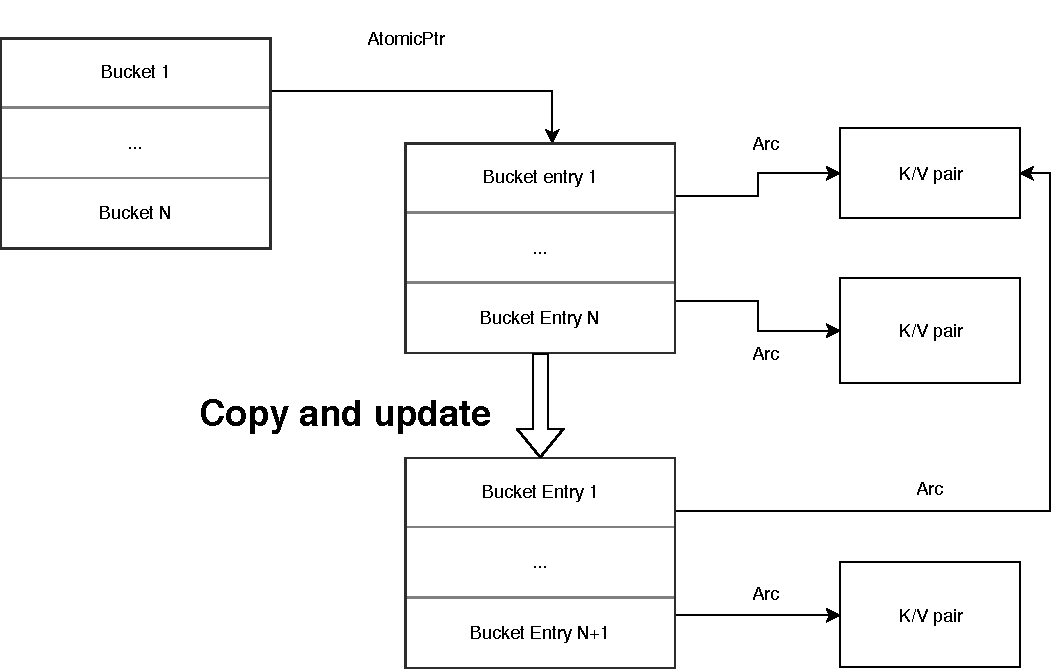
\includegraphics[width=\textwidth]{../diagram/amap2.pdf}
  \caption{Value insertion}
  \label{fig:omvcc-insert}
\end{figure}

This lock-free design allows a fast, concurrent and zero-copy
insertion of values inside the hashmap. However in the case where the
workload is write-heavy, an optimistic concurrency control scheme will
result in a lot of wasted work as each thread will need to build
the new version of the bucket multiple times. The most expensive
operation for an insert is actually the atomic compare and swap. Since
a typical workload on key-value stores implies a majority of reads
compared to writes (the Facebook USR load is only 0.2\%
writes~\cite{memcached}), this won't be a problem in our target use
case.

If we consider all the properties that the resulting hashmap
has, we realize that it uses an optimistic multi-version concurrency
control scheme. Optimistic, since each thread works on its own before
attempting to synchronize with other threads, and multi-version since
each bucket can have multiple versions in use at any given point.

\begin{figure}
  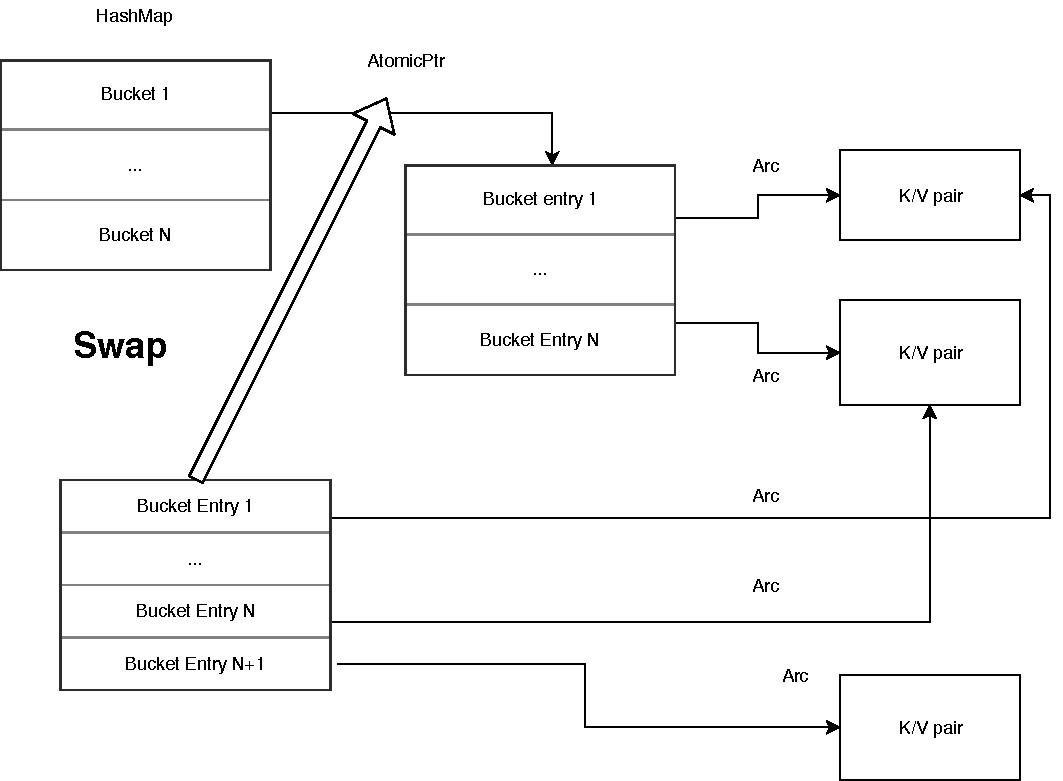
\includegraphics[width=\textwidth]{../diagram/amap3.pdf}
  \caption{Bucket swapping}
  \label{fig:omvcc-swap}
\end{figure}

\begin{figure}[htb!]
  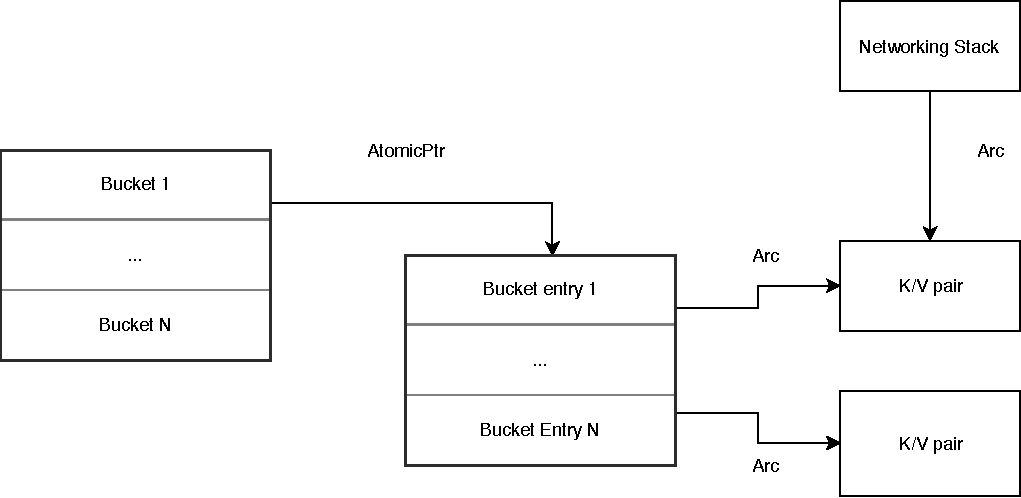
\includegraphics[width=\textwidth]{../diagram/cc2.pdf}
  \caption{Concurrent value removal}
  \label{fig:cc2}
\end{figure}

On a related note, Rust's concurrency guarantees ensure that sharing
key-value pairs extracted from the hashmap amongst threads isn't a
problem. Indeed since each thread will have an immutable reference to
the data, the compiler will enforce that these threads don't modify it
at compile time.

\section{Key-value store}

The key-value store is what would be considered as the user
application. As such it will provide an example of how to use the
system. It is the last layer of the system and should not rely on any
details of the lower layers of the networking stack. Its role in the
system while be to process individual R2P2 request and parse them
using the application layer protocol.

\section{R2P2 stack}

As stated in the design goals the R2P2 stack should provide an
easy-to-use, reliable and zero-copy interface to user
applications. This R2P2 stack is the interface between the user
application itself (the key-value store in our case) and the UDP
networking stack and handles request parsing, response sending and
retransmissions when needed.

The R2P2 stack will be implemented on top of the UDP stack described in
section~\ref{sec:udp-design}. The API design of the R2P2 stack is
therefore constrained by the design of the UDP stack. We thus make use
of callback in the R2P2 stack. The R2P2 stack itself interfaces with
the UDP stack by registered a callback invoked on each UDP
packet. Since R2P2 provides multi-packet requests, the R2P2 should
handle reconstruction of requests. Since the user application will
only care about handling complete requests the R2P2 stack will store
packets and group by them by request and finally invoke the user
provided callback once the whole request has been received and
parsed. This callback should construct the response from the
request. The R2P2 stack then handles transmitting the response to the
client using the UDP stack.

The R2P2 layer is also responsible for the reliable delivery of
responses. It should then hold on to responses produced by the user
callback until they are acknowledged by the clients. In order to avoid
duplicating work, and thereby reducing both latency and throughput,
it should also identify when a request has already been processed by
the user application and avoid processing this request again.

\section{UDP stack} \label{sec:udp-design}

The core of this project is not the low level details of interfacing
with a NIC or even the kernel bypass. We will thus use an existing
framework to do that for us and build our networking on top of said
framework.

It is worth mentioning the Linux kernel socket flag for zero copy.
Though it does not provide guaranteed zero copy sending/receiving a
port of nginx using it saw a 9\% increase in performance with minimal
code changes. The choice was made not to use it, since it would
eliminate one of the most interesting aspect of the project, the
ability to have a safe userspace networking stack in the same address
space as the user program.

As for the local store, the UDP stack should uphold the zero-copy
property of the system. That means it should interface with the
kernel-bypassing framework and extract data from that framework while
not copying anything.

Kernel bypassing frameworks follow what is known as a run to
completion model, the driver polls the NIC for incoming
packets~\cite{dpdk-pmd} and hands them over to the user application in
batches. This will influence the API design of the UDP stack and
forbid the classic socket style API typically found in kernel
networking stacks. Since we aim to provide a convenient and safe Rust
API to the UDP stack we will need to come up with an alternative
design.

The run to completion model thus prompts a callback based API
design. We thus have a callback oriented UDP stack. Since the
framework polls the NIC for packets on its own this is
appropriate. When the user application creates a new socket on the
stack, it will provide a closure. Once a packet is received, its
headers will be parsed and the UDP stack will dispatch to the
appropriate socket registered earlier by the user application. Of
course the callback provided by the user application should be
reentrant since it will potentially be invoked from many threads
concurrently.


%%% Local Variables:
%%% mode: latex
%%% TeX-master: "master"
%%% End:
